\chapterimage{water}
\chapter{Performance analysis}\label{sec:rate_distortion}

The goal of this chapter is to present the main performance metrics
(objective and subjective) employed to evaluate lossless and lossy compression pipelines.

\section{Spacetime}\label{sec:rate_distortion:rate}

\conceptRef{lossless compression}{Lossless} compression pipelines are relatively straightforward to analyze.
By definition, they preserve all information and allow a perfect reconstruction of the original data. Therefore, the compressed data size and required computational resources typically offer sufficient insight.

One of the most useful metrics to assess compressed data size is the \concept{compressed data rate},
expressed in \concept{bits per sample} (bps), and defined simply as
$\displaystyle \frac{\textrm{compressed data size (bits)}}{\textrm{number of original samples}}$.
Depending on the context, the generic term ``sample'' is substituted by the specific sample type.
For instance, the term \concept{bits per pixel} (bpp) is used in image compression,
whereas \concept{bits per base} (bpb) is used in DNA sequence compression.

\begin{remark}
In the context of image compression, sometimes the term ``\concept{pixel}'' refers to a spatial position $(x,y)$. For \conceptRef{color image}{color} and \concept{multispectral} images that have multiple \conceptRef{band}{bands}, there are multiple samples at each spatial position.
%
To prevent potential ambiguity, one can use the \concept{bits per pixel per component} (bpppc)
and even bits per sample so that each $(x,y,z)$ position is considered a separate sample.
\end{remark}

One advantage of the bits per sample metric is an easy comparison with the source's entropy $\entropy(\source)$.
This way, it is easy to compute the \concept{efficiency} of a compression pipeline,
defined as $\displaystyle \eta = \frac{\entropy(\source)}{\textrm{bits per sample}}$.

Another popular metric for assessing compression performance is the \concept{compression ratio}.
This is often defined as $\displaystyle \textrm{CR} = \frac{\textrm{original data size}}{\textrm{compressed data size}}$ and requires no units.
%
With this definition, if compression compacts data to half the original size,
the compression ratio would be $2$, or equivalently $2:1$. Although simple, this metric has some potential pitfalls:
\begin{itemize}
\item Some authors define compression ratio as the inverse of the above definition. In the previous example,
the compression ratio would be $1/2$ instead of $2$.
\item The ``original data size'' is sensitive to the way they are originally stored. Some factors that may affect this value are:
\begin{itemize}
    \item the bitdepth of the raw representation,
    \item the presence or absence of headers, and
    \item the original data be available in an already compressed format.
\end{itemize}
\end{itemize}

Another critical dimension for evaluating compression pipelines is the required computational resources. Of particular importance are \conceptRef{compression time}{compression/decompression time} and \concept{memory usage}. Compression time is particularly important in contexts such as \concept{remote sensing} because of the limited time to process each sample, but also because time is a good surrogate metric to battery usage.
%
Other derived metrics exist to evaluate compression speed, \eg \concept{throughput},
that combine execution time and the number of samples compressed.

To properly evaluate compression time, it is necessary to run multiple executions for each sample.
After that, the \concept{average}, \concept{median} and \concept{minimum} statistics can be used
to summarize the measurements, although a distribution analysis can be even more informative.

\section{Distortion}

Lossy compression pipelines permit almost arbitrary compressed data size reductions,
easily outperforming lossless schemes in that regard. However, this is at the cost
of introducing some degree of distortion in the reconstructed data.
%
In order to properly evaluate lossy compression, the compressed file size
and the introduced distortion must be analyzed simultaneously.
This \concept{rate-distortion analysis} be performed for instance with a 2D plot
such as the following one:

\begin{center}
    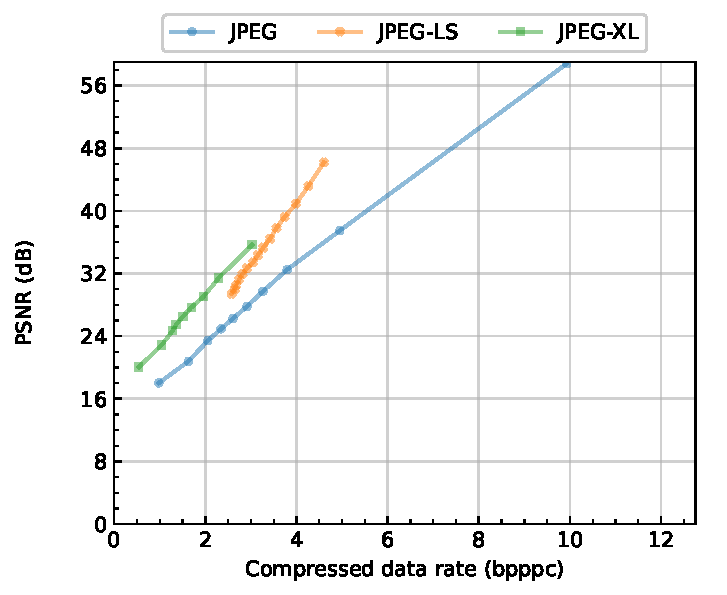
\includegraphics[width=0.5\linewidth]{rate_distortion_plot}
\end{center}

\begin{itemize}
\item The $x$ axis displays a metric of compressed data size (\eg, the compressed data rate).
\item The $y$ axis displays a metric of distortion (see some options below).
\item Each marker in the plot corresponds to one compression pipeline with one specific set of parameters.
    The different markers of the same pipeline are often linked with a line for better clarity.
\item For a test \concept{corpus} with more than one sample (\eg, more than one image),
    the $x$ and $y$ values can be the average rate and distortion across the corpus.
    It is also possible to include insight on the dispersion ``hidden'' by each marker
    (\eg, displaying $\pm 1$~standard deviation, or plotting a point of clouds instead of a single
    line per pipeline).
\end{itemize}

Rate-distortion plots allow quick comparison of different pipelines. In particular,
they can help determine what pipeline yields a lower distortion (higher \concept{fidelity})
for a given rate, and what pipeline achieves a certain quality with the smallest compressed
data volumes.

A key element of these plots is the choice of \concept{distortion metric} for the $y$ axis.
These metrics can be \conceptRef{objective distortion metric}{objective}
or \conceptRef{subjective distortion metric}{subjective}.
Objective metrics perform a deterministic computation using the original $X$ and
the reconstructed $\hat{X}$ data. Subjective metrics, on the other hand, require
humans to give their opinion on their perceived quality of the reconstructed data.

Most objective distortion metrics are directly linked to
physical signal notions (such as \concept{error power}). Some of the most relevant
are listed next~\cite[\S 8.1]{sayood_introduction}:
\begin{itemize}
    \item the \concept{mean squared error} (MSE),
    \item the \concept{peak signal-to-noise ratio} (PSNR),
    \item the \concept{peak absolute error} (PAE), and
    \item the \concept{spectral angle} (hyperspectral imagery~\cite[``The Spectral Angle Mapper (SAM)'']{kruse_spectral_angle}).
\end{itemize}

While useful~\cite{mse_love}, the metrics above do not directly take into account the
\concept{psychovisual} and \concept{psychoacoustic} properties of humans, so they often
fail to predict the results of subjective distortions. Other metrics have been developed
to address this problem, involving more or less complex models of the human sensory systems, including:
\begin{itemize}
\item the \concept{structural similarity} (SSIM~\cite{wang_ssim}),
\item the \concept{multiscale structural similarity} (MS-SSIM~\cite{wang_ms_ssim}) metrics, and
\item the HDR-VDP-3 metric~\cite{mantiuk2023hdr}.
\end{itemize}

If interested, make sure to request a full presentation on \concept{perceptual coding}
from your closest data compression professor.


\section*{Further reading and practice}

\begin{itemize}
\item Sayood's book~\cite[\S 8.3]{sayood_introduction} offers a very clear overview of the most popular
distortion criteria.

\item Taubman and Marcellin's book~\cite{taubman2002jpeg2000} contains a brief but nice introduction to information irrelevance in \S 1.2.2,
part of which is further developed in \S 4.3.4 and 16.1.

\item This paper~\cite{mse_love} provides invaluable insight and food for thought
on the most popular distortion metric in many areas of data compression (MSE).
\end{itemize}

\begin{exercise}
What's the minimum and maximum efficiency $\eta$ achievable by a scalar entropy coder?
How about a complete compression pipeline?
\end{exercise}

\begin{exercise}
Provide matemathical expressions for the objective distortion metrics
based on physical signal properties mentioned in this chapter.
\end{exercise}

\begin{exercise}
Find the distortion metrics used in these papers, paying close attention to the way results are presented:
\begin{enumerate}[label=\alph*)]
\begin{multicols}{4}
    \item \cite{auli_llinas_visuallylossless}
    \item \cite{maireles_gonzalez_astro}
    \item \cite{bartrina_ccsds}
    \item \cite{chow_k2raster}
    \item \cite{tzamarias_runlength}
    \item \cite{verdu_mijares_hyperspectral}
    \item \cite{fan_probability}
    \item \cite{veller_tans}
    \item \cite{bartrina_ccsdsreview}

  \item \cite{martin_lostsignals}
  \item \cite{zeghidour_soundstream}
  \item \cite{marpe_mpeglowcomplexity}
  \item \cite{kim_svacencoder}
  \item \cite{li_dnacompression}
  \item \cite{liu_lossyqualityvalues}
  \item \cite{huang_clusteringdna}
  \item \cite{de_moura_waveletecg}
  \item \cite{mao_ecg_lzw}
  \item \cite{rodriguez_lasvas}
  \item \cite{li_transformvvc}
\end{multicols}
\end{enumerate}

\end{exercise}

\begin{exercise}
Rank the compression time of the entropy coders you used in Chapter~\ref{sec:coding}
for the \url{mandrill-u8be-3x512x512.raw} image. Also provide the throughput in each case.
\end{exercise}

\begin{exercise}
Perform your own rate-distortion analysis using the mandrill image and at least
two lossy compressors. For instance, you can use the JPEG and JPEG-LS codecs
available at \url{https://github.com/thorfdbg/libjpeg/}.
\end{exercise}
